\documentclass[t, xcolor=dvipsnames]{beamer}

\usepackage[utf8]{inputenc}
\usepackage[T1]{fontenc}
\usepackage{fontspec}
\usepackage{helvet}
\usepackage[english]{babel}
\usepackage{verbatim}

\setsansfont{Rotis}[
	Extension   = .otf ,
	UprightFont = *-Regular ,
	BoldFont    = *-Bold ,
	ItalicFont  = *-Italic
]

\usetheme{LUH}



\title{Basics of Bash}
\date[26.10.2023]{26.10.2023}
\author[Seidl, de Vries]{Barbara Seidl, Jan de Vries, Steffen Weßbecher}
\unilogo{
\includegraphics[height=\LUHLogoHeight]{LUH}}
\logo{
\includegraphics[height=\LUHLogoHeight]{logo}}
\titleimage{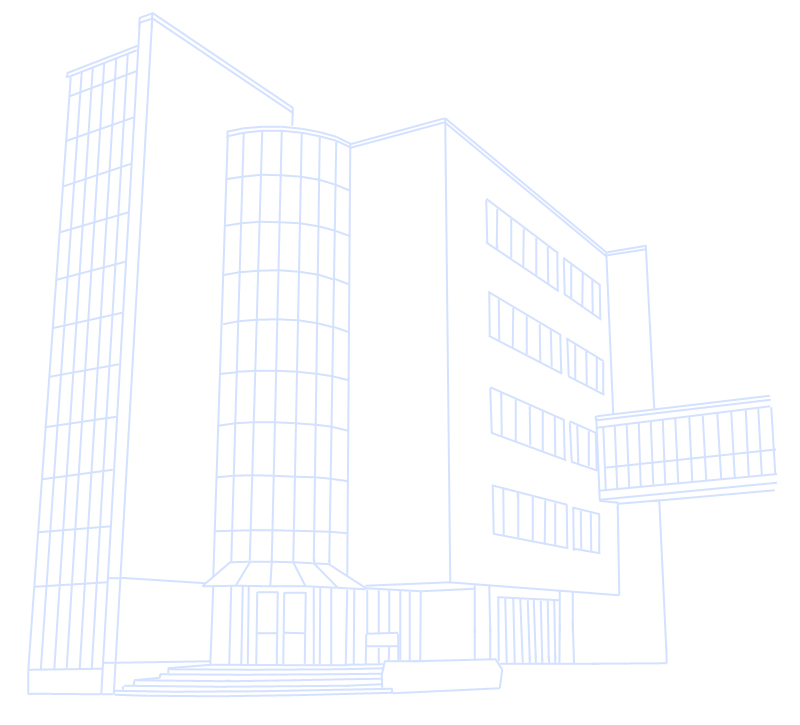
\includegraphics[width=.35\paperwidth]{appel-strasse}}



\begin{document}

\begin{frame}
\titlepage

\begin{columns}
	% Column 1
	\begin{column}{0.5\textwidth}
	
	\end{column}
	% Column 2    
	\begin{column}{0.5\textwidth}
	Oder: How to feel like Hackerman
	\begin{figure}
    	\centering
    	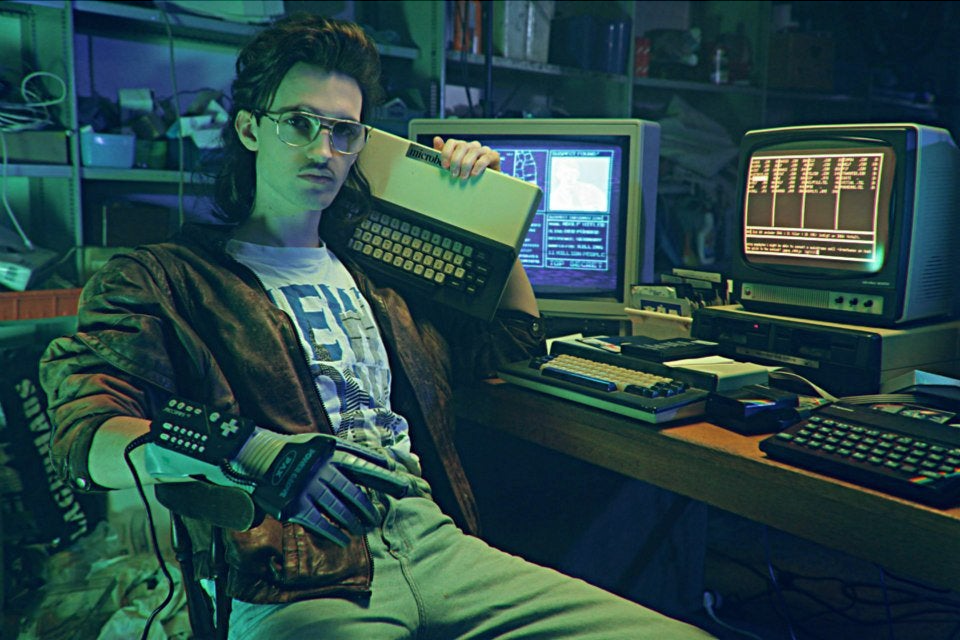
\includegraphics[width=1\textwidth]{graphics/hackerman}
        	\tiny{Quelle: Kung Fury\\ \#schaut den Film, er ist sehr gut!\\ Los tut es!}
    	\end{figure}
    	
	\end{column}
\end{columns}

\end{frame}



\begin{frame}{Was machen wir hier eigentlich?}{ (..und warum machen wir das?) }


\begin{itemize}
    \item Vorteile der Kommandozeile (Hacker sehen immer so cool aus..)
    \item Umgang mit der Konsole
    \item Orientierung im Unix/Linux System
\end{itemize}

\begin{columns}
    \begin{column}{0.5\textwidth}
    \begin{figure}
        \centering
        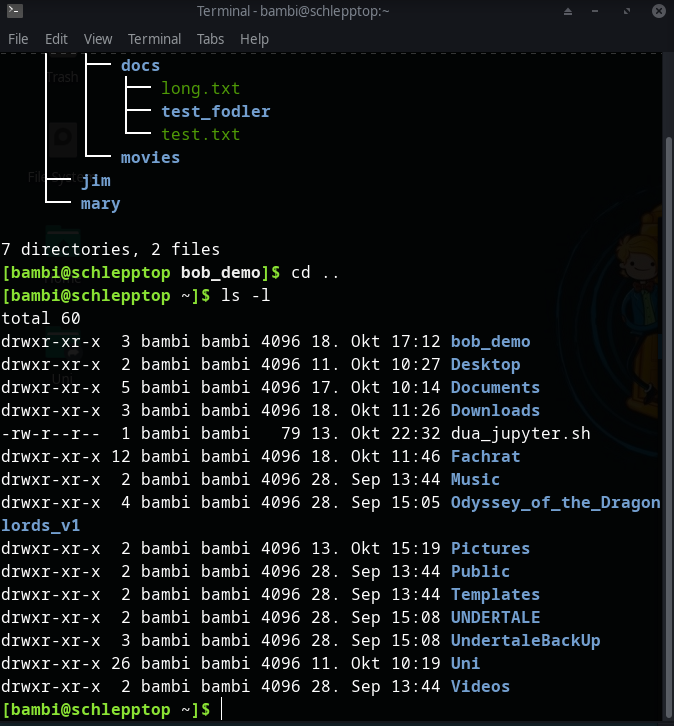
\includegraphics[width=1.0\textwidth]{graphics/terminal}
    \end{figure}
    \end{column}
    
    \begin{column}{0.5\textwidth}
    \begin{figure}
        \centering
        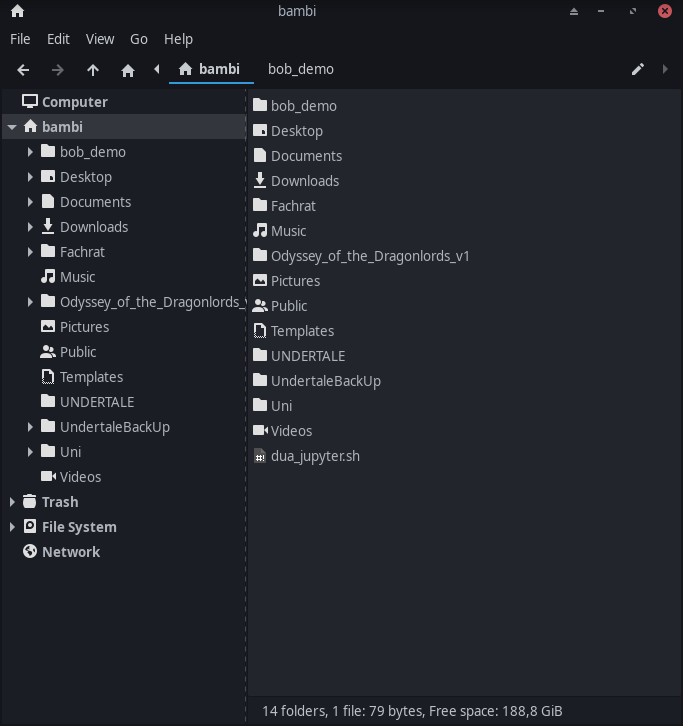
\includegraphics[width=1.0\textwidth]{graphics/klicki-bunti}
    \end{figure}
    \end{column}
    
\end{columns}
  
\end{frame}



\begin{frame}{So könnte eure Konsole aussehen\dots}
Was sehen wir hier?

\begin{figure}
    \centering
    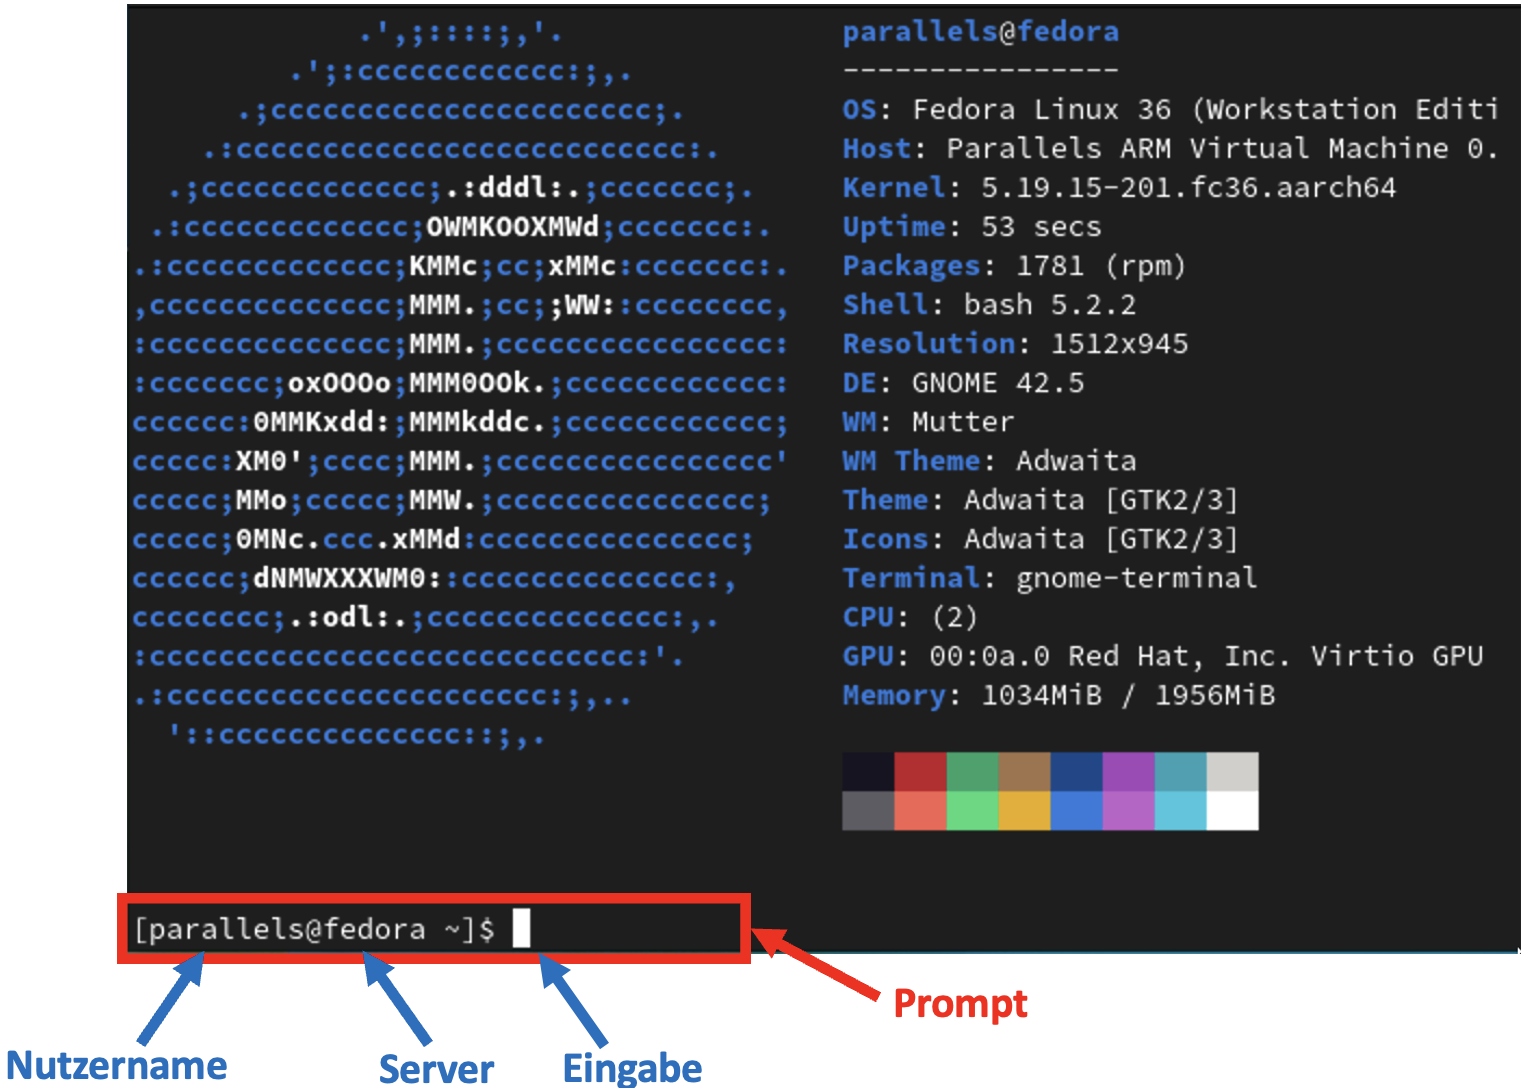
\includegraphics[width=0.75\textwidth]{graphics/prompt}
\end{figure}

\end{frame}

\begin{frame}{Der Dateibaum}

    \begin{itemize}
        \item \textcolor{blue}{Absoluter Pfad}: Von der Wurzel
        \item \textcolor{red}{Relativer Pfad}: Von deiner Position
    \end{itemize}

    \begin{columns}
	% Column 1
	\begin{column}{0.65\textwidth}
\begin{figure}
    \centering
    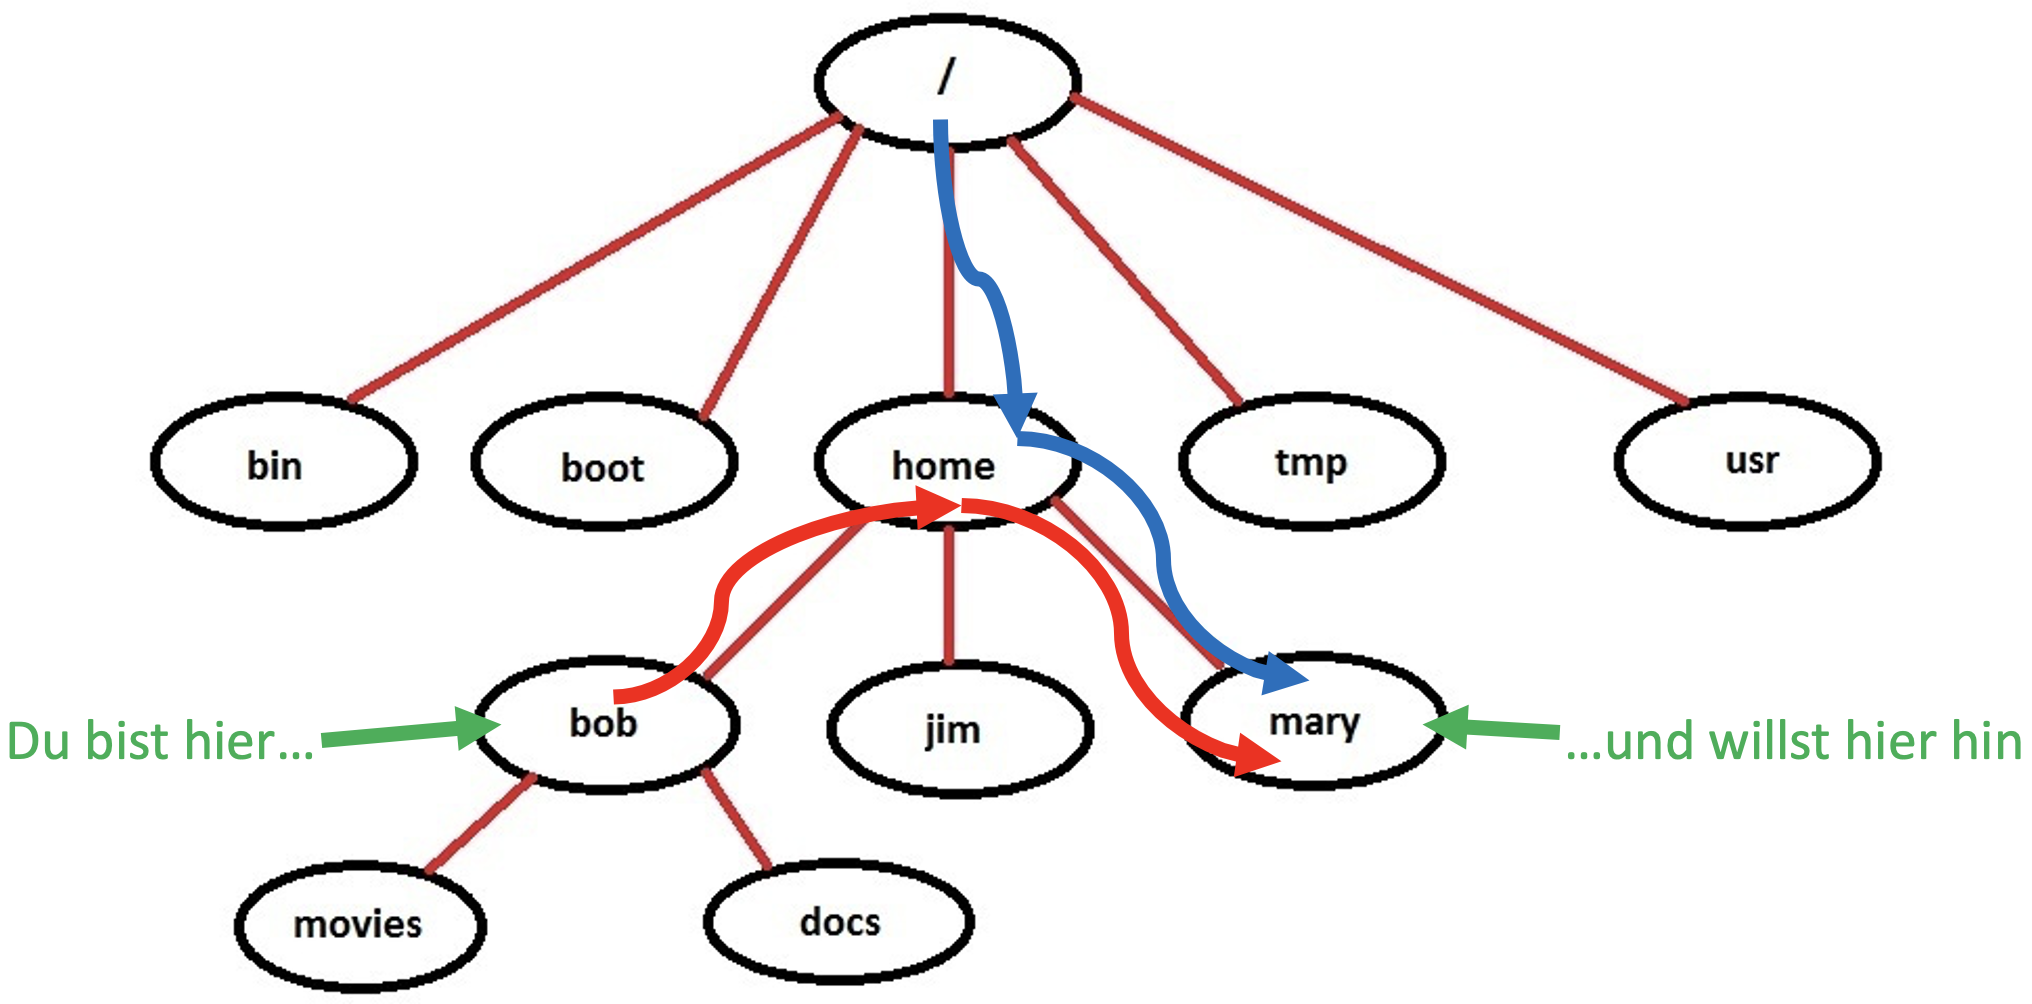
\includegraphics[width=1\textwidth]{graphics/dateipfad}
\end{figure}
	\end{column}
	% Column 2    
	\begin{column}{0.35\textwidth}
	
	    \begin{block}{}
	       \begin{itemize}
	           \item Dein Home: \textasciitilde
	           \item Aktueller Ordner: .
	           \item Ordner über dir: ..
	       \end{itemize}
	    \end{block}
    	
	\end{column}
\end{columns}
    
\end{frame}

\begin{frame}{Wo bin ich und wie komme ich woanders hin?}
    \begin{columns}
        % Column 1
	    \begin{column}{0.7\textwidth}
	        \begin{itemize}
	            \item Dein aktueller Pfad: \textcolor{blue}{pwd}
	            \item In einen Ordner wechseln: \textcolor{blue}{cd}
	            \item Ordner werden mit "/" getrennt. Man kann durch angeben eines Pfades also größere Sprünge machen
	        \end{itemize}
	        
	    \end{column}
	    % Column 2    
	    \begin{column}{0.3\textwidth}
	
	    % Zur Erinnerung:
	    \begin{block}{}
	       \begin{itemize}
	           \item Dein Home: \textasciitilde
	           \item Aktueller Ordner: .
	           \item Ordner über dir: ..
	       \end{itemize}
	    \end{block}
    	
    	
    	
	    \end{column}
    \end{columns}
    
    \begin{figure}
	        \centering
	        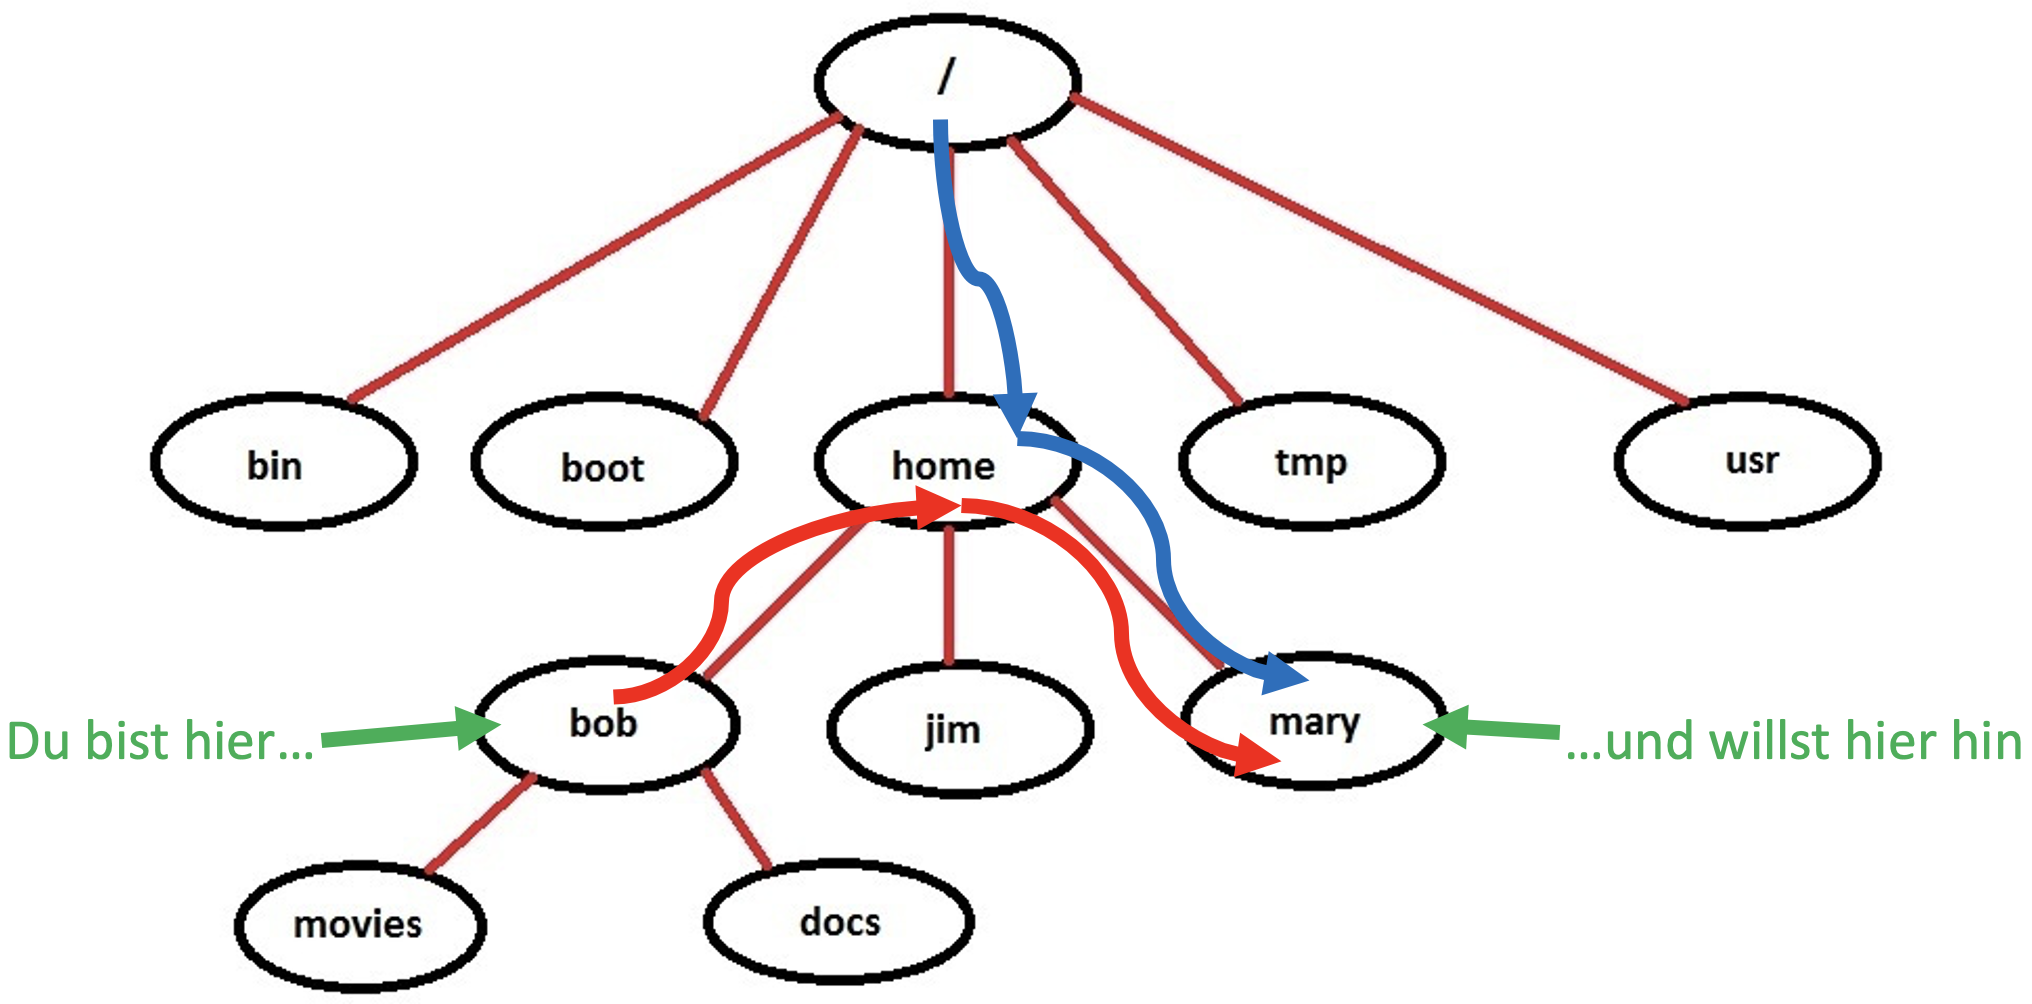
\includegraphics[width=0.5\textwidth]{graphics/dateipfad}
	\end{figure}
    
\end{frame}

\begin{frame}{Beispiel \textcolor{blue}{cd}}
    \begin{columns}
        \begin{column}{0.5\textwidth}
            %\begin{itemize}
             %   \item \textcolor{blue}{pwd}: \textcolor{red}{/home/bob}
	          %  \item \textcolor{blue}{cd ..}
	           % \item \textcolor{blue}{pwd}: \textcolor{red}{/home}
	            %\item \textcolor{blue}{cd mary}
	            %\item \textcolor{blue}{pwd}: \textcolor{red}{/home/mary}
            %\end{itemize}
            
            \begin{itemize}
                \item \textcolor{ForestGreen!70!Black}{Du bist hier (\textcolor{blue}{pwd}):} /home/bob
                \item \textcolor{ForestGreen!70!Black}{.. und willst hier hin (\textcolor{blue}{pwd})}: /home/mary
            \end{itemize}
            \begin{figure}
	        \centering
	        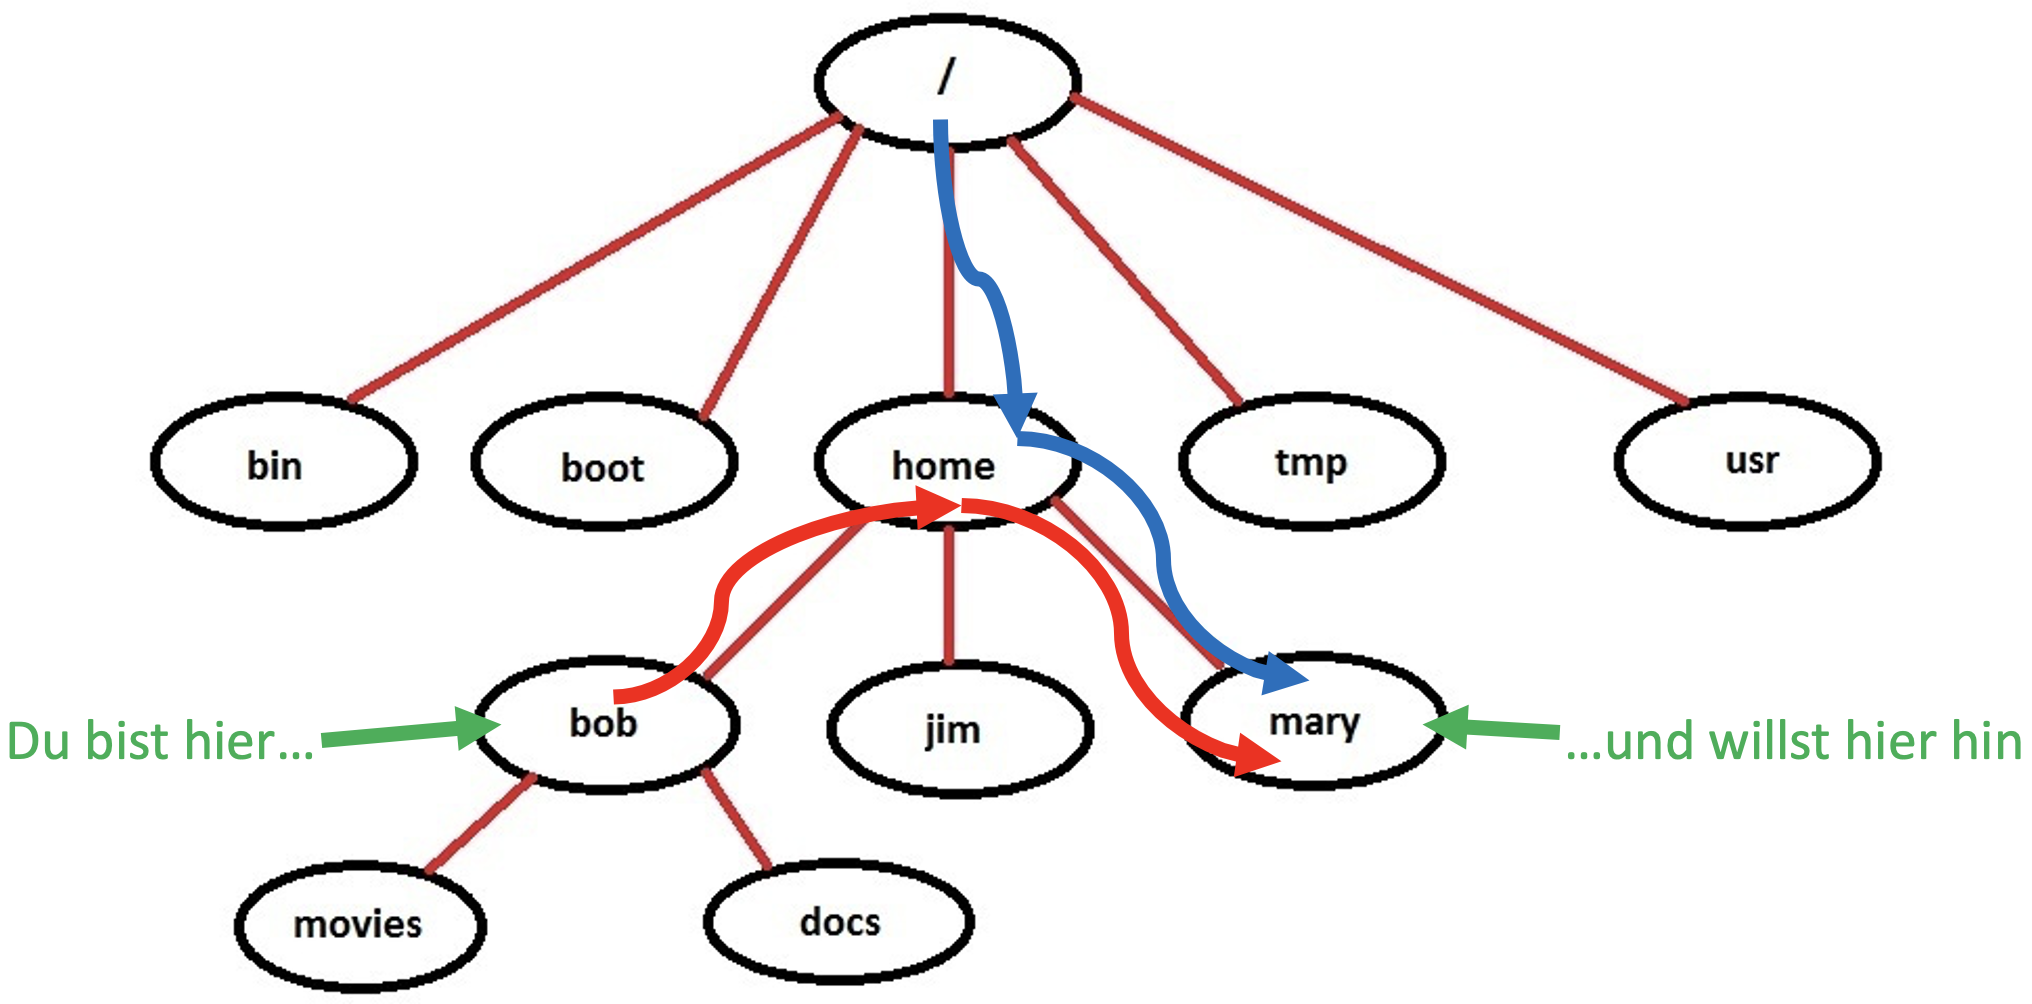
\includegraphics[width=0.9\textwidth]{graphics/dateipfad}
	\end{figure}
        \end{column}
        \begin{column}{0.5\textwidth}
        
            Entweder:
            \begin{itemize}
                \item \textcolor{blue}{cd} \textcolor{RoyalBlue!80}{/home/mary}
            \end{itemize}
           
           Oder:
           \begin{itemize}
               \item \textcolor{blue}{cd} \textcolor{red}{../mary}
           \end{itemize}
            %Alternativ:
            %\begin{itemize}
            %    \item \textcolor{blue}{pwd}: \textcolor{red}{/home/bob}
            %    \item \textcolor{blue}{cd ../mary}
            %    \item \textcolor{blue}{pwd}: \textcolor{red}{/home/mary}
            %\end{itemize}
            %Oder:
            %\begin{itemize}
            %    \item \textcolor{blue}{pwd}: \textcolor{red}{/home/bob}
            %    \item \textcolor{blue}{cd \textasciitilde/mary}
            %    \item \textcolor{blue}{pwd}: \textcolor{red}{/home/mary}
            %\end{itemize}
            
        \end{column}
    \end{columns}
    
    
	
	
\end{frame}

\begin{frame}{Ist in dem Ordner was drin?}
    \begin{itemize}
        \item Den Inhalte eines Ordners anzeigen: \textcolor{blue}{ls} oder \textcolor{blue}{ls} \textcolor{orange}{<ordner>}
        % \item Geht das auch übersichtlicher? Ja!: \textcolor{blue}{ls -l}
    \end{itemize}
    
    \begin{figure}
        \centering
        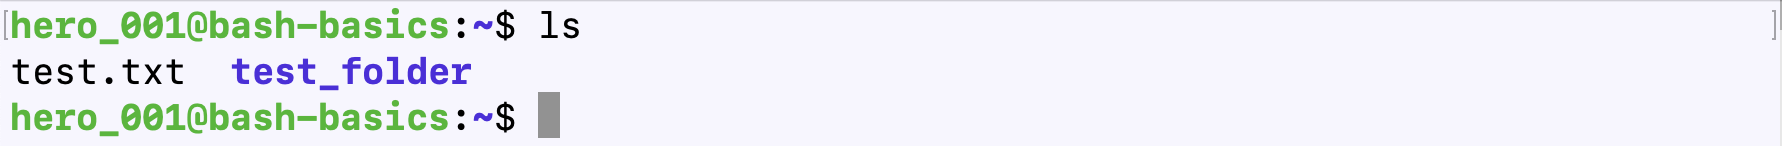
\includegraphics[width=1\textwidth]{graphics/ls}
    \end{figure}
    
    %\begin{figure}
    %    \centering
    %    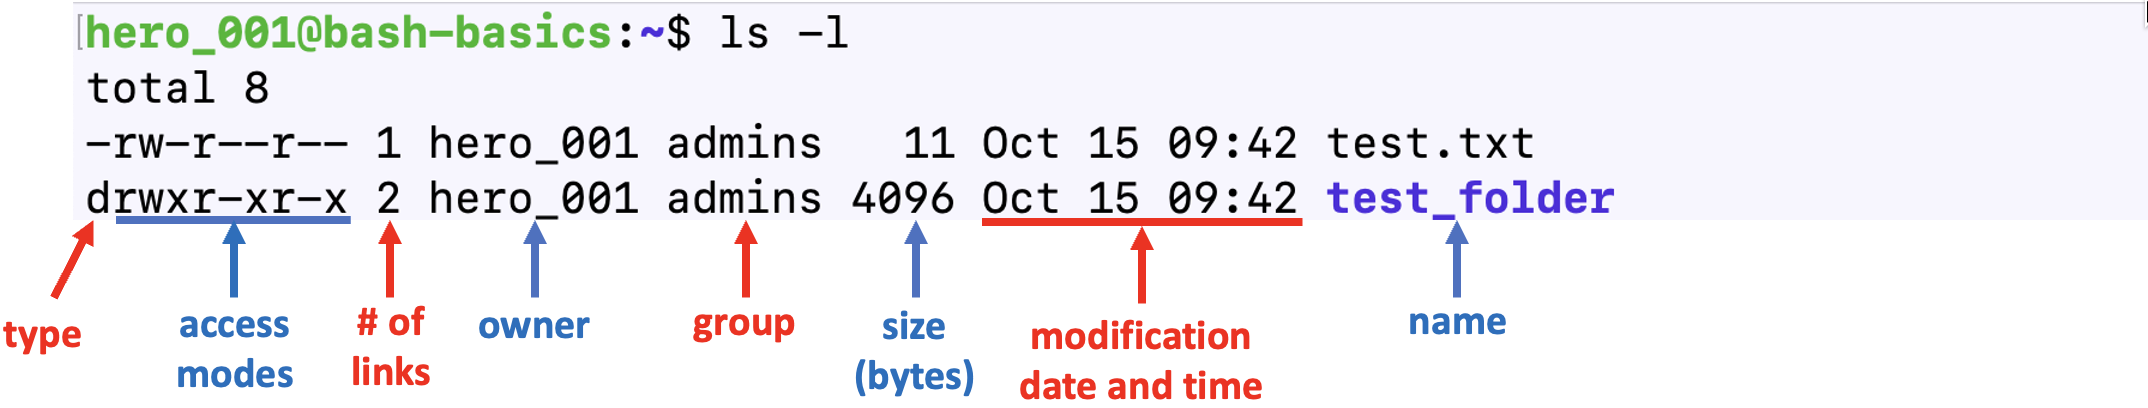
\includegraphics[width=1\textwidth]{graphics/ls -l explained}
    %\end{figure}
\end{frame}

\begin{frame}{Ist in dem Ordner was drin? Teil 2}
    \begin{itemize}
        \item Den Inhalte eines Ordners anzeigen: \textcolor{blue}{ls} oder \textcolor{blue}{ls} \textcolor{orange}{<ordner>}
        \item Geht das auch übersichtlicher? Ja!: \textcolor{blue}{ls -l}
    \end{itemize}
    
    \begin{figure}
        \centering
        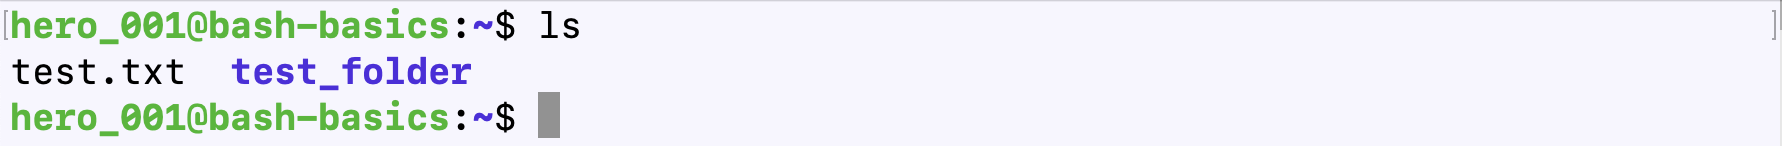
\includegraphics[width=1\textwidth]{graphics/ls}
    \end{figure}
    
    \begin{figure}
        \centering
        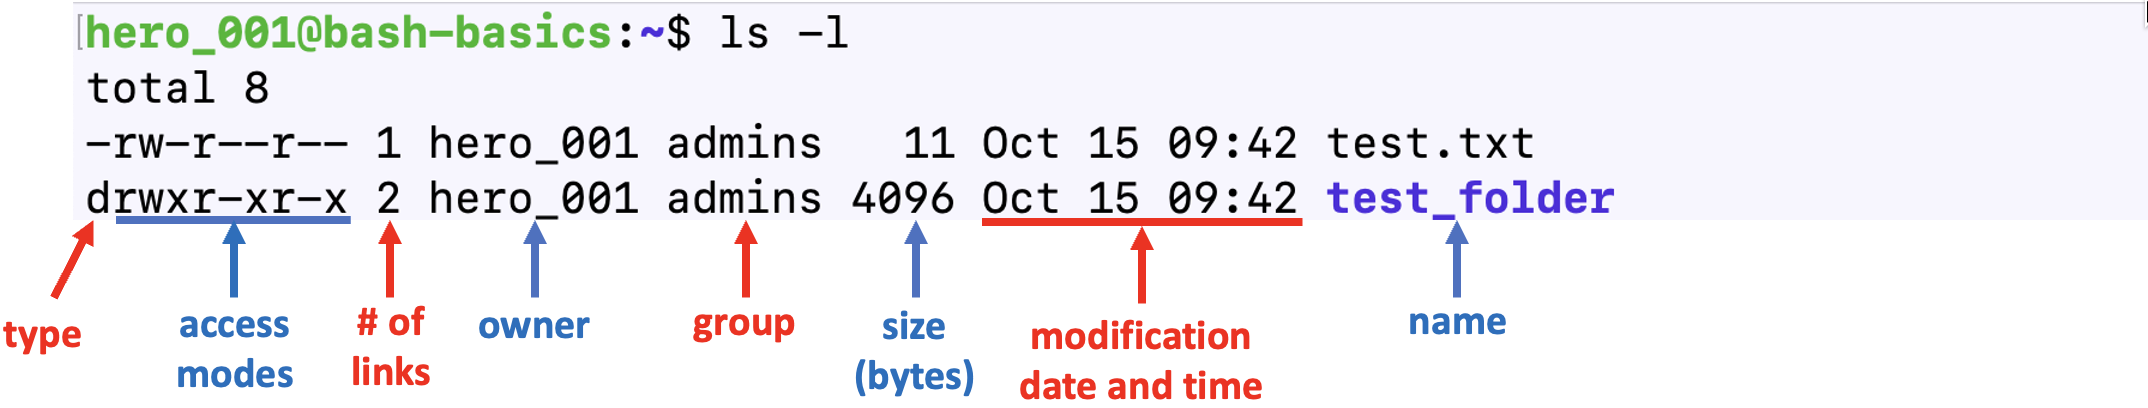
\includegraphics[width=1\textwidth]{graphics/ls -l explained}
    \end{figure}
\end{frame}

\begin{frame}{Rechteverwaltung (\textcolor{blue}{chmod})}

    \begin{columns}
	% Column 1
	\begin{column}{0.5\textwidth}
	
	\begin{itemize}
        \item Eingabe:\\ \textcolor{blue}{chmod} \textcolor{orange}{<mode> <datei>}
        \item Mode besteht aus drei Zahlen\\z.B. "\textcolor{teal}{736}"\\ \, \, \, \, \ \textcolor{red}{ugo}\\ u = Besitzer; g = Gruppe;\\ o = Andere
        \item Bsp: \textcolor{blue}{chmod} \textcolor{teal}{764} test.txt
    \end{itemize}
	
	\end{column}
	% Column 2    
	\begin{column}{0.5\textwidth}
	
	\begin{table}[]
        \begin{tabular}{|c|l|c|}
            \hline
            \textbf{\#} & \textbf{Berechtigung} & \textbf{rwx}\\
            \hline
            \textcolor{teal}{7} & Voll & 111 \\
            \hline
            \textcolor{teal}{6} & Lesen und Schreiben & 110 \\
            \hline
            \textcolor{teal}{5} & Lesen und Ausführen & 101 \\
            \hline
            \textcolor{teal}{4} & Nur Lesen & 100 \\
            \hline
            \textcolor{teal}{3} & Schreiben und Ausführen & 011 \\
            \hline
            \textcolor{teal}{2} & Nur Schreiben & 010 \\
            \hline
            \textcolor{teal}{1} & Nur Ausführen & 001 \\
            \hline
            \textcolor{teal}{0} & Keine & 000 \\
            \hline
        \end{tabular}
    \end{table}
    	
	\end{column}
\end{columns}
    
\end{frame}


\begin{frame}{Manual (\textcolor{blue}{man})}
    \begin{itemize}
        \item Ihr wisst mal nicht, was genau ein Befehl macht? \\ Nutzt einfach \textcolor{blue}{man} \textcolor{orange}{<komischer Befehl>}
        \item Exit mit \textcolor{blue}{q}
    \end{itemize}
    
    \begin{figure}
        \centering
        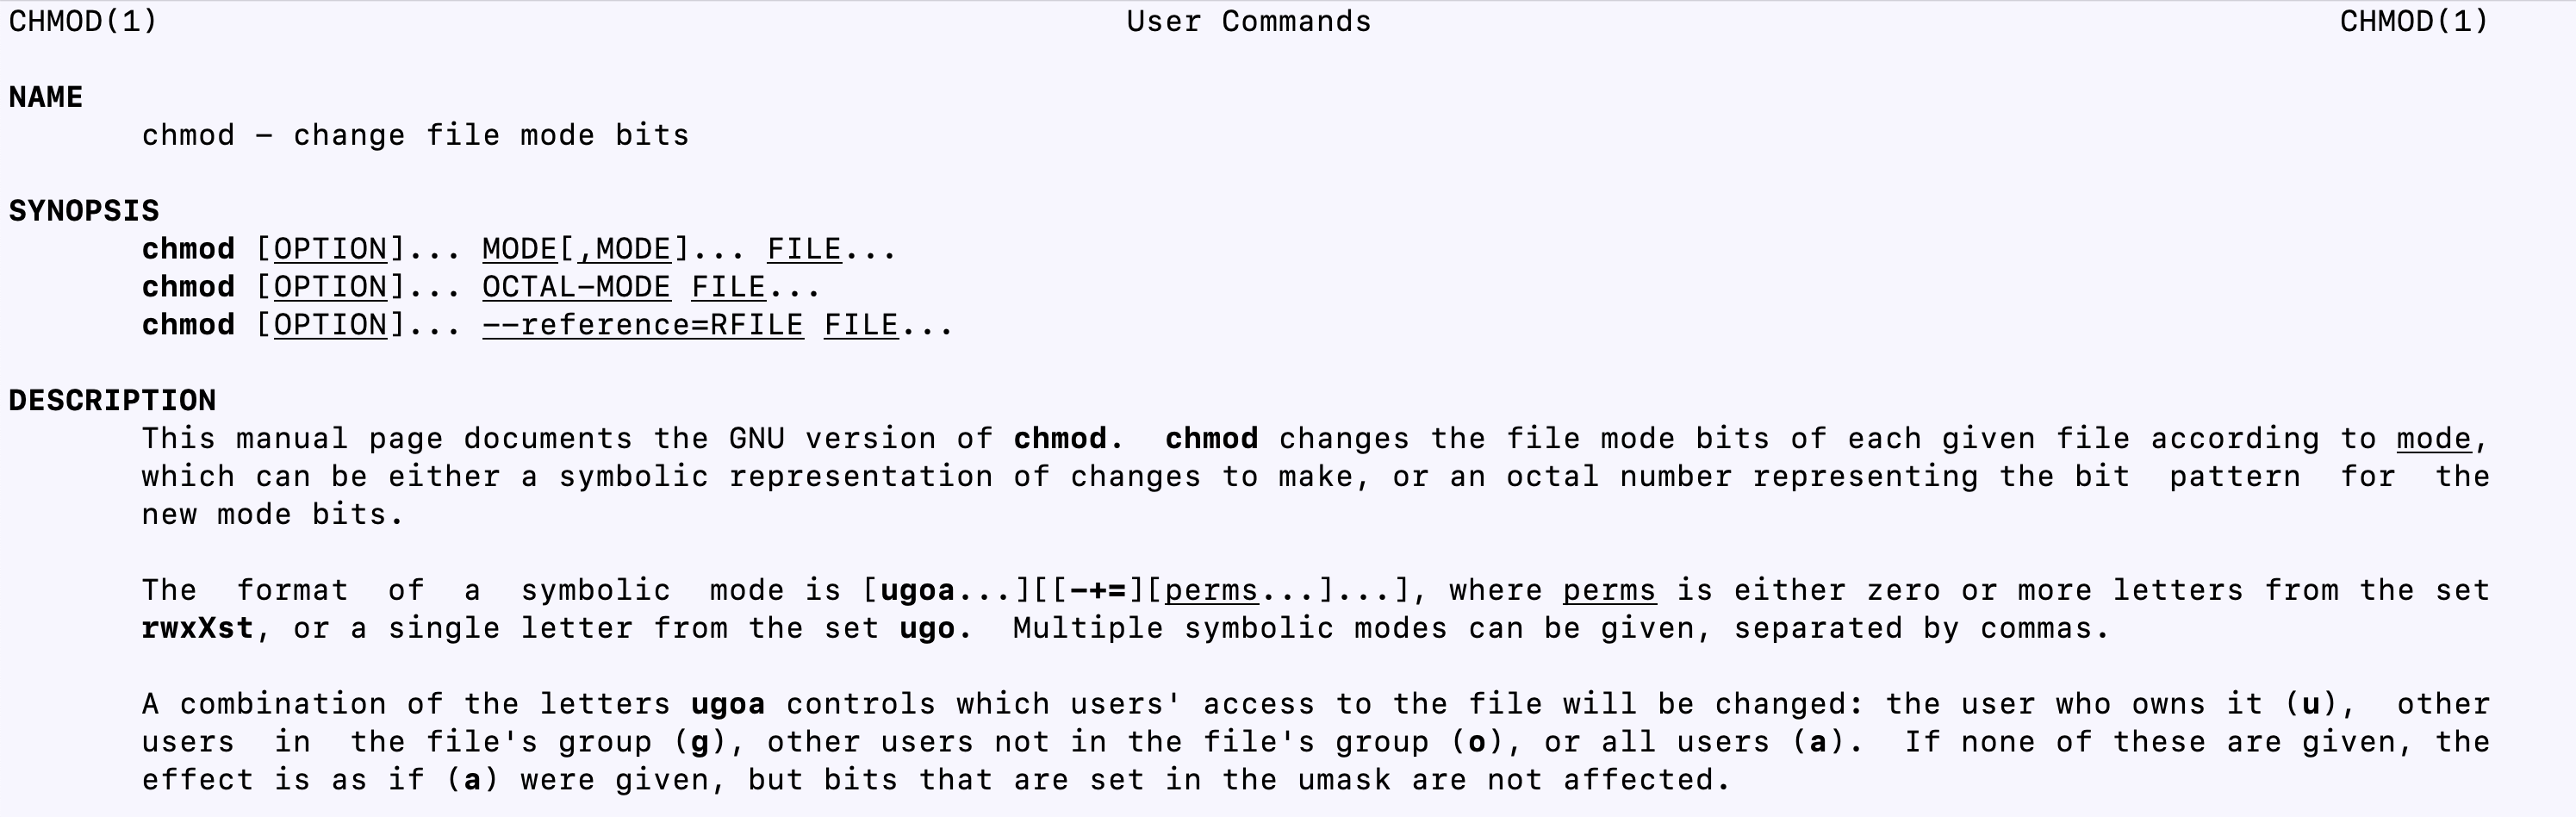
\includegraphics[width=1\textwidth]{graphics/man}
    \end{figure}
\end{frame}

\begin{frame}{Dateiinhalte anzeigen}
    \begin{itemize}
        \item Ganzen Inhalt einer Datei anzeigen: \textcolor{blue}{cat} \textcolor{orange}{<datei>}
        \item Inhalt temporär anzeigen (\textcolor{blue}{q} zum Beenden): \textcolor{blue}{less} \textcolor{orange}{<datei>}
        \item Anfang einer Datei: \textcolor{blue}{head} \textcolor{orange}{<datei>}
        \item Ende einer Datei: \textcolor{blue}{tail} \textcolor{orange}{<datei>}
    \end{itemize}
    
    \begin{figure}
        \centering
        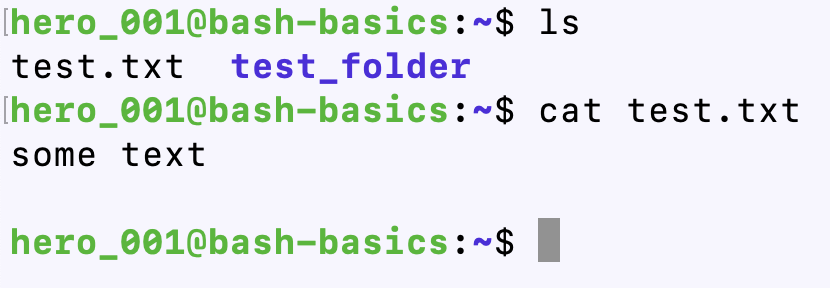
\includegraphics[width=0.7\textwidth]{graphics/cat}
    \end{figure}
\end{frame}

\begin{frame}{Suchen}
	\begin{itemize}
		\item Eine Datei suchen: \textcolor{blue}{find} \textcolor{orange}{<Startordner>} \textcolor{blue}{-name "}\textcolor{orange}{<Name>}\textcolor{blue}{"}
        \item Den Inhalt aller Dateien in einem Ordner durchsuchen:\\ \textcolor{blue}{grep "}\textcolor{orange}{<Suchwort>}\textcolor{blue}{"} \textcolor{orange}{<Ordner>}
        \item \textcolor{blue}{grep -r} \textcolor{blue}{(\dots)} für eine rekursive Suche vom \textcolor{orange}{<Startordner>} "abwärts"
	\end{itemize}
	\begin{figure}
		\centering
		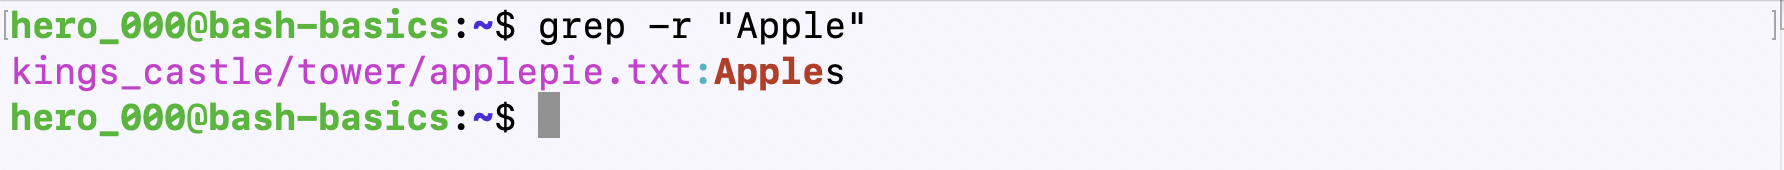
\includegraphics[width= 1\textwidth]{graphics/grep}
	\end{figure}
\end{frame}

\begin{frame}{Bearbeiten}
    \begin{itemize}
        \item Eine Datei bearbeiten/erzeugen: \textcolor{blue}{nano} \textcolor{orange}{<datei>}
        \begin{itemize}
            \item Speichern mit: \textcolor{teal}{Strg + o}
            \item Verlassen mit: \textcolor{teal}{Strg + x}
            \item \textcolor{red}{(Gegebenenfalls Dialog beachten)}
        \end{itemize}
    \end{itemize}
    
    \begin{figure}
        \centering
        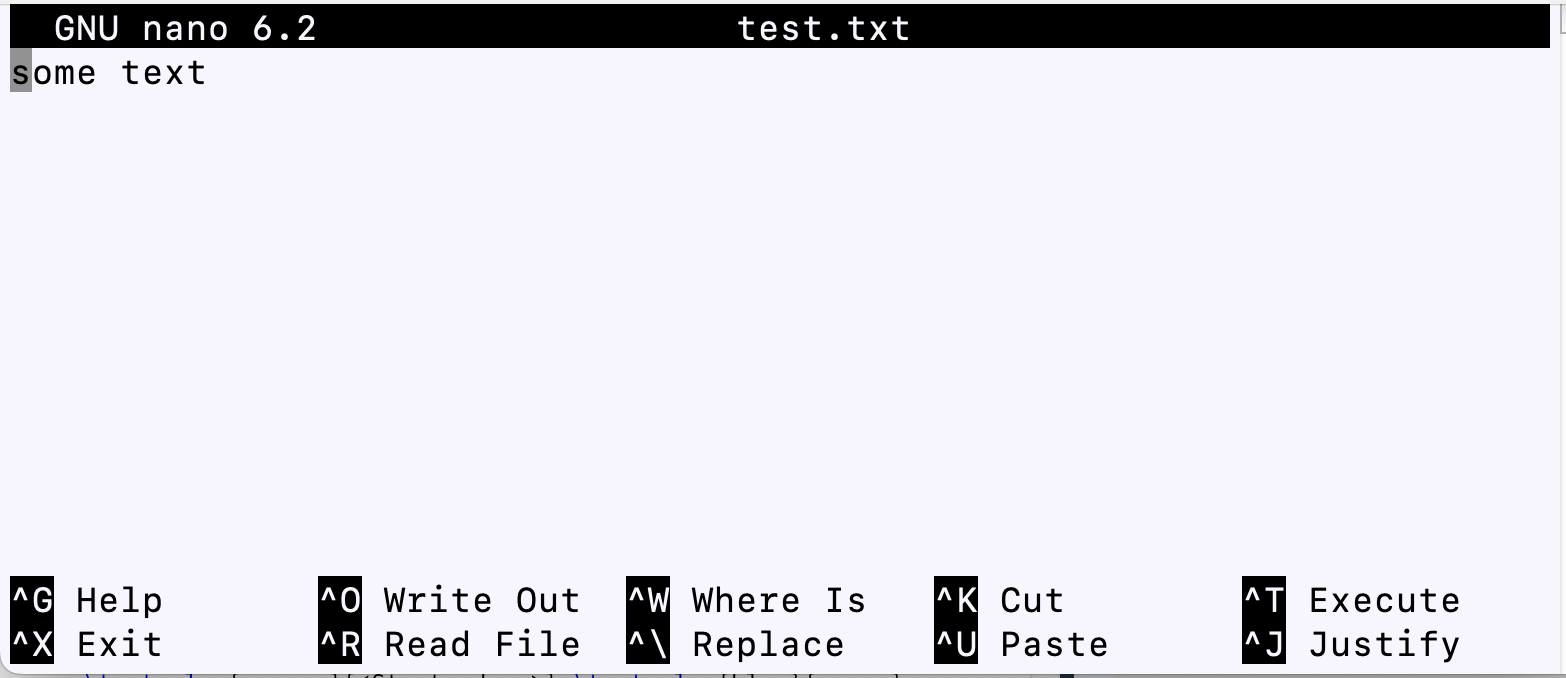
\includegraphics[width=0.55\textwidth]{graphics/nano}
    \end{figure}
    
    \begin{itemize}
    	\item Die ultra krassen dürfen Vim nutzen (\textcolor{blue}{vim }\textcolor{orange}{<datei>}) \#EscapeTheVim
    \end{itemize}
\end{frame}

\begin{frame}{Weitere nützliche Befehle}
    \begin{itemize}
        \item Ordner erstellen: \textcolor{blue}{mkdir} \textcolor{orange}{<Ordnername>}
        \item Dateien löschen: \textcolor{blue}{rm} \textcolor{orange}{<datei>}
        \item Ordner mit Inhalt löschen: \textcolor{blue}{rm -r} \textcolor{orange}{<datei>}
        \item Datei kopieren: \textcolor{blue}{cp} \textcolor{orange}{<datei> <Zielpfad/Neue\_Datei>}
        \item Datei verschieben oder umbenennen: \textcolor{blue}{mv} \textcolor{orange}{<datei> <Zielpfad>}
    \end{itemize}
    
    \begin{figure}
    	\centering
    	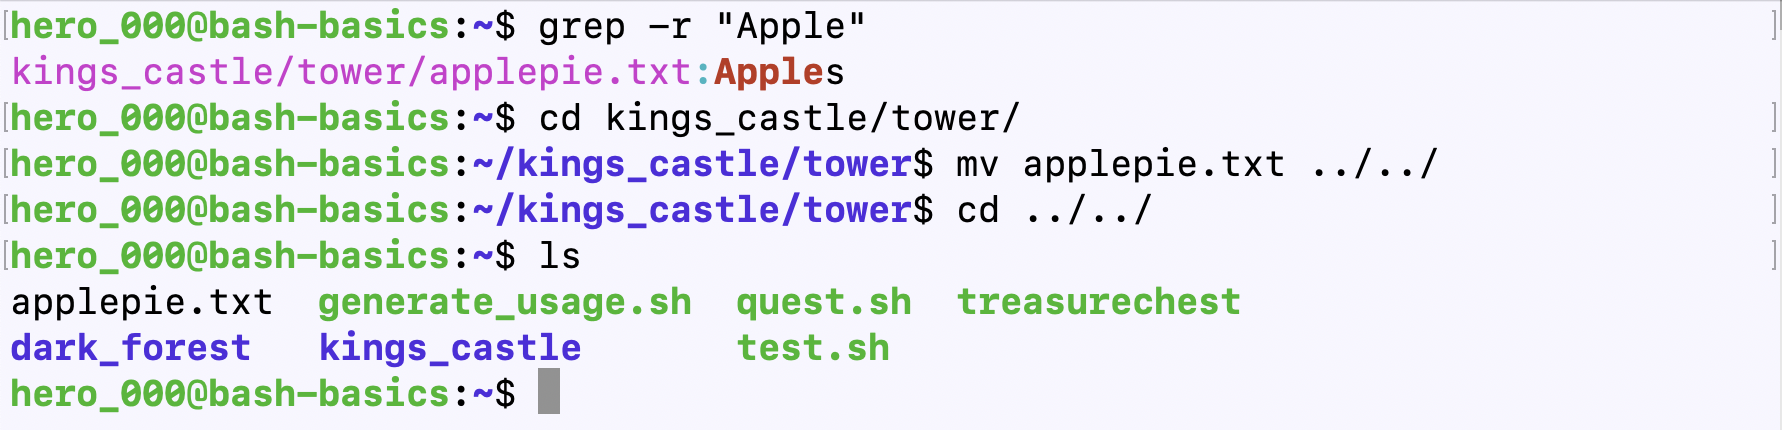
\includegraphics[width=1\textwidth]{graphics/mv}
    \end{figure}
\end{frame}


\begin{frame}{How to SSH}
    \begin{itemize}
        \item Mit lokalen Netzwerk verbinden:
        \begin{itemize}
            \item Netzwerkname: \textcolor{blue}{BashBasicsBroadcast}
            \item Kennwort: \textcolor{blue}{bootebooteboote}
        \end{itemize}
        \item Öffne dein Terminal
        \item Eingabe: \textcolor{blue}{ssh hero\_}\textcolor{orange}{<deine Nummer>}\textcolor{blue}{@basics-of-bash}
        \item Passwort = Nutzername (das was vor dem "@" steht)
        \item Passwort ändern: \textcolor{blue}{passwd}
        \item Disconnect: \textcolor{blue}{exit}
    \end{itemize}
    \begin{figure}
        \centering
        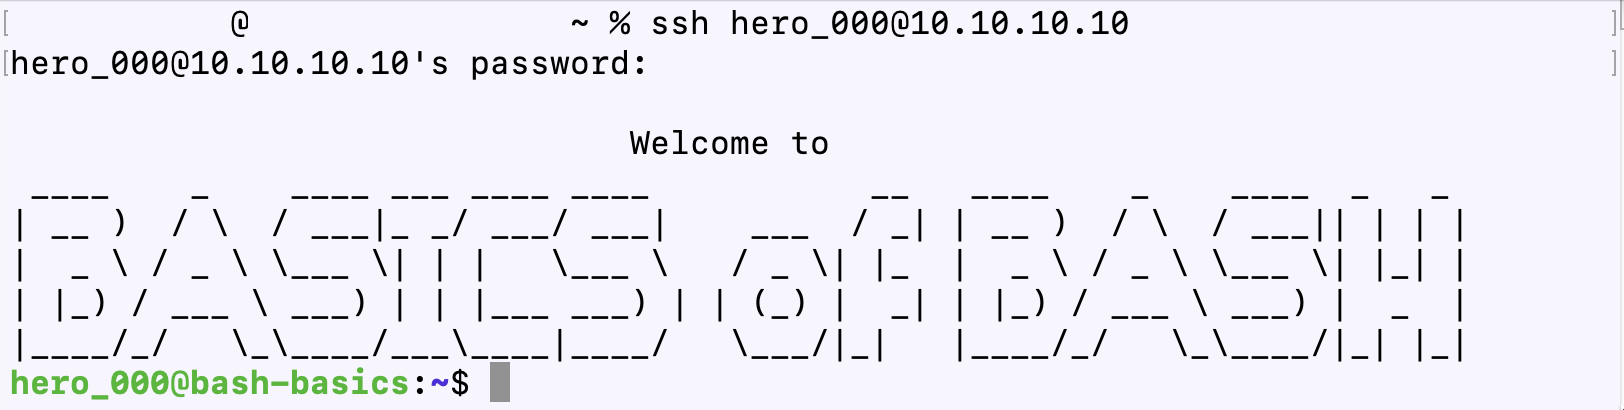
\includegraphics[width=1\textwidth]{graphics/ssh}
    \end{figure}
\end{frame}

\begin{frame}{Damit könnt ihr starten}
    \begin{itemize}
        \item Seht euch eure Quest an: \textcolor{blue}{./quest.sh} oder \textcolor{blue}{bash quest.sh}
        \item Weitere Tipps: 
        \begin{itemize}
            \item Mit TAB könnt ihr z.B. Pfade automatisch vervollständigen lassen
            \item \textcolor{blue}{*} ist ein "Wildcard"-Symbol \\
            Wenn ihr also einen Dateinamen nicht vollständig kennt:\\
            \textcolor{blue}{find} \textcolor{orange}{<Startordner>} \textcolor{blue}{-name "*}\textcolor{orange}{<Teilname>}\textcolor{blue}{*"}
        \end{itemize}
        
    \end{itemize}
\end{frame}

\begin{frame}{Cheat-Sheet für den Workshop}
    \begin{itemize}
        \item Ein Shell-Skript ausführen: \textcolor{blue}{./} oder \textcolor{blue}{bash} \textcolor{orange}{<datei>.sh}
        \item Inhalt einer Datei anzeigen: \textcolor{blue}{cat} \textcolor{orange}{<datei>}
        \item Aktueller Pfad: \textcolor{blue}{pwd}
        \item Den Ordner wechseln: \textcolor{blue}{cd}
        \item Inhalt anzeigen lassen: \textcolor{blue}{ls}
        \item Eine Datei suchen: \textcolor{blue}{find} \textcolor{orange}{<Startordner>} \textcolor{blue}{-name "}\textcolor{orange}{<Name>}\textcolor{blue}{"}
        \item \textcolor{blue}{*} ist ein "Wildcard"-Symbol \\
        \textcolor{blue}{find} \textcolor{orange}{<Startordner>} \textcolor{blue}{-name "*}\textcolor{orange}{<Teilname>}\textcolor{blue}{*"}
        \item Dateiinhalt durchsuchen: \textcolor{blue}{grep -r "}\textcolor{orange}{<Suchwort>}\textcolor{blue}{"} \\ \textcolor{blue}{-r}: Suche setzt sich rekursiv durch alle Unterordner fort
        %\item Datei verschieben: \textcolor{blue}{mv} \textcolor{orange}{<datei> <Zielpfad>}
        \item Mit TAB könnt ihr z.B. Pfade automatisch vervollständigen lassen
        \item Datei kopieren: \textcolor{blue}{cp} \textcolor{orange}{<datei> <Zielpfad/Neue\_Datei>}
        \item Datei verschieben: \textcolor{blue}{mv} \textcolor{orange}{<datei> <Zielpfad>}
    \end{itemize}
\end{frame}


\begin{frame}{\huge{Feedback ist gerne erwünscht!}}
    \vspace{5mm}
    \normalsize
    \begin{itemize}
        \item \textcolor{blue}{cd \textasciitilde/../feedback}
        \item \textcolor{blue}{nano } \textcolor{orange}{<lustiger\_dateiname>.txt}
        \item Type your Feedback
        \item Verlassen und Speichern: \textcolor{teal}{Strg o, Strg + x}\\ \textcolor{red}{(Dialog beachten!)}
    \end{itemize}
    
\end{frame}

\begin{frame}{Was habt ihr heute gelernt?}
\begin{itemize}
    \item Wie man sich ein kleines bisschen wie Hackerman fühlt
    \item Sich per SSH auf einem Server einloggen
    \item Ordner wechseln
    \item Neue Ordner und Dateien erstellen
    \item Dateien verschieben, kopieren und bearbeiten
    \item Dateien durchsuchen
\end{itemize}

\vspace{15mm}
    \huge{Vielen Dank!}
    
\end{frame}

\begin{frame}{Weitere Angebote des FR Inf}
    \begin{figure}
        \centering
        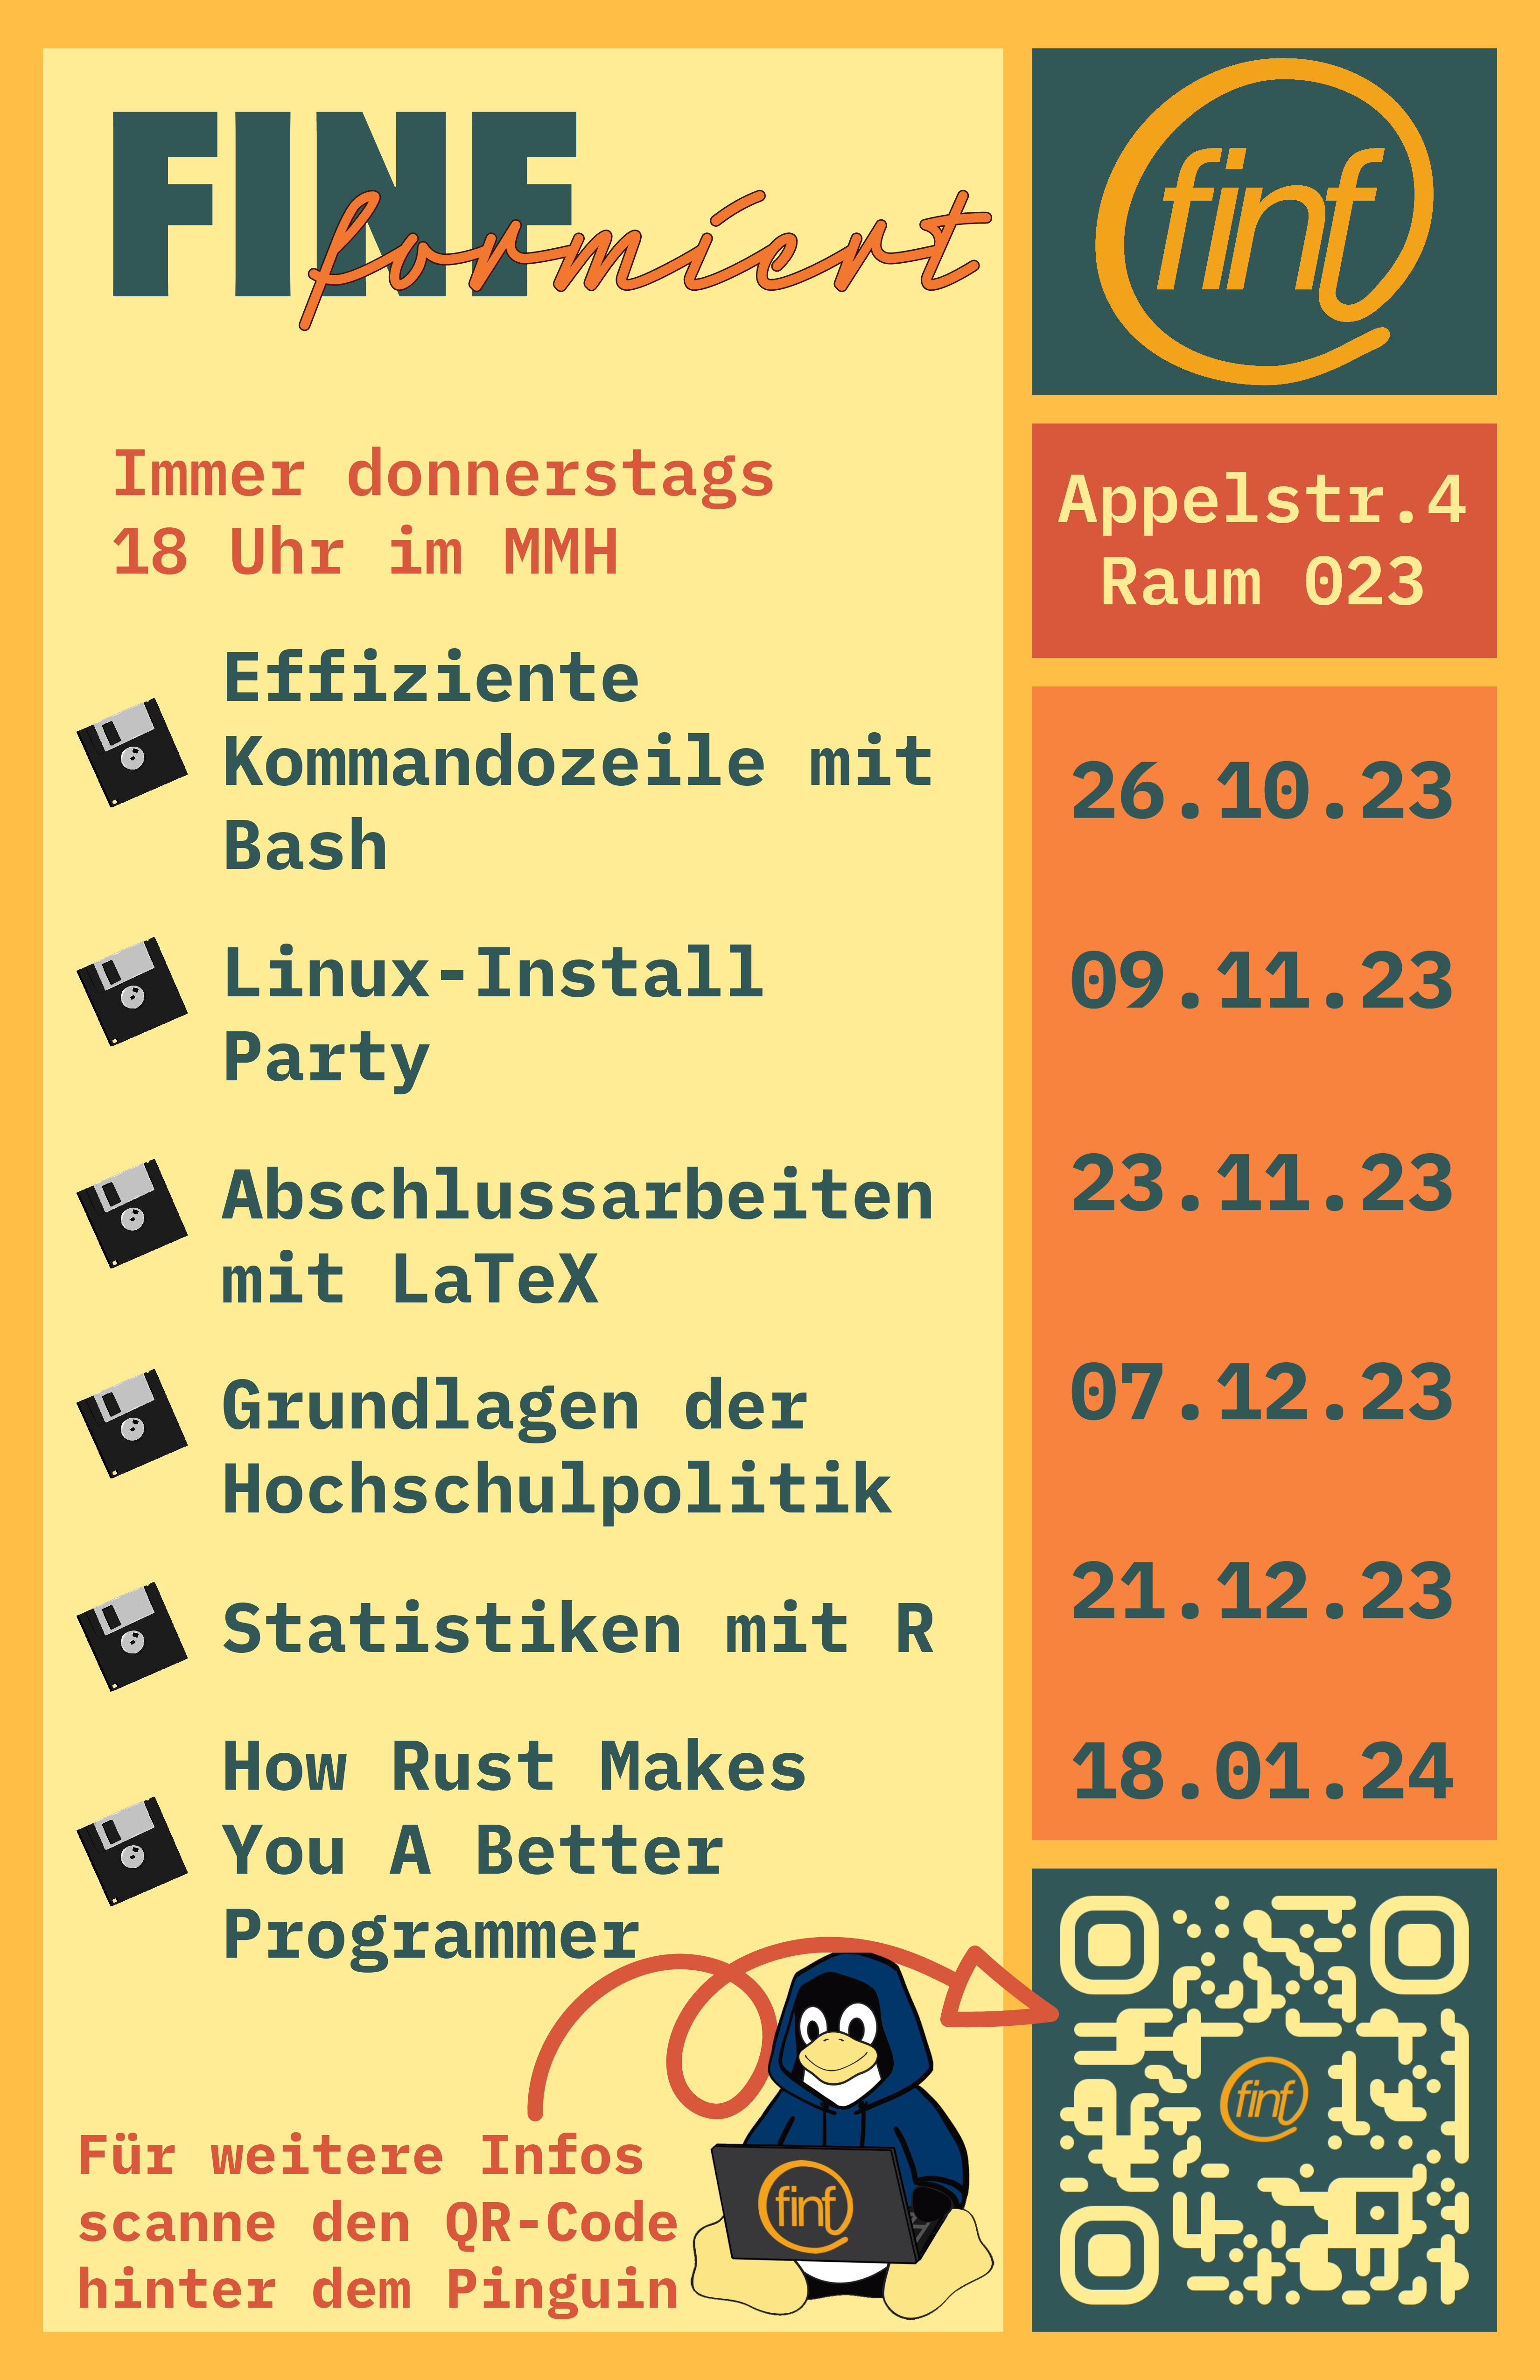
\includegraphics[width=0.38\textwidth]{basicsofbash/graphics/finformiert Poster 2023 v8.png}
    \end{figure}
\end{frame}

\end{document}
